\documentclass{article}
\usepackage{graphicx} % Required for inserting images
\usepackage[top=0.9in, bottom=1in, left=1.5in, right=1.5in]{geometry}
\usepackage[utf8]{inputenc}
\usepackage[icelandic]{babel}
\usepackage[T1]{fontenc}
\usepackage[sc]{mathpazo}
\usepackage[parfill]{parskip}
\renewcommand{\baselinestretch}{1.2}
% Tables and lists
\usepackage{booktabs,tabularx}
\usepackage{multirow}
\usepackage{enumerate}
\usepackage{adjustbox}
\usepackage{multicol}
\usepackage{xcolor}
\usepackage{algpseudocode}
\usepackage{tikz}
\usepackage{nicefrac}
\usepackage{changepage}
\usetikzlibrary{arrows, positioning, calc, graphs}

% Math
\usepackage{amsmath, amsfonts, amssymb, amsthm}
% Graphics

\usepackage{graphicx}
\usepackage{tikz}
% Code environment
\usepackage{minted}
%\usepackage{bm}
%\usepackage{siunitx}
%\usepackage{animate}
%\usepackage{hyperref}
%\usepackage{movie15}
%\usepackage{multicol}
%\usepackage{changepage}
\title{Formal Languages and Computability 1}
\author{Ragnar Björn Ingvarsson, rbi3}
\tikzset{->, >=stealth', shorten >=1pt, node distance=2cm,thick, main node/.style={circle,draw,minimum size=3em}}


\begin{document}
\renewcommand\thepage{}
	
	\maketitle

	\newpage
	\setcounter{page}{1}
	\renewcommand\thepage{\arabic{page}}
	\section{Let $t_{i+1} = (2t_i - 1)^2$. Show by induction that $0 \leq
	t_i \leq 1$ for all \textit{i} if $0 \leq t_0 \leq 1.$}

	We notice that the base case $0 \leq t_0 \leq 1$ has already been 
	provided, therefore we continue with $k \in \mathbb{N}$ where we 
	assume $0 \leq t_k \leq 1$.

	We notice that $2t_k$ results in \[0 \leq 2t_k \leq 2\] and then 
	\[-1 \leq 2t_k - 1 \leq 1\]

	Now squaring $2t_k - 1$ will give a range between $0$ and $1$ since 
	it will not be negative and the lowest number it can give is $0$ where 
	$t_k = \nicefrac{1}{2}$. Therefore:

	\[0 \leq (2t_k - 1)^2 \leq 1\]

	And since we have the precondition $t_{i+1} = (2t_i - 1)^2$ we get

	\[0 \leq t_{k+1} \leq 1\]

	$\hfill\blacksquare$


	\section{Draw a state diagram for a DFA that \textit{accepts} any 
		binary string that has three or more consecutive 
	zeroes.}

	Here we simply need to have three ladder-like states where each 
	consecutive $0$ brings you to the next one, but each $1$ knocks 
	you all the way down. If then, we get three consecutive zeroes we 
	get locked to the fourth state where the string can continue with any 
	number of zeroes or ones and then end at any time.

	\begin{center}

	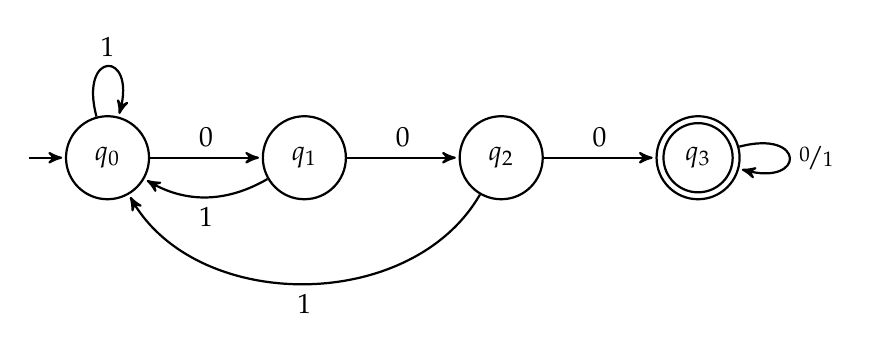
\begin{tikzpicture}[thick, auto]
		\node[main node] (A) {$q_0$};
		\node[main node] at (2.5,0) (B) {$q_1$};
		\node[main node] at (5,0) (C) {$q_2$};
		\node[main node] at (7.5,0) (D) {$q_3$};
		\node[main node, minimum size=2.5em] at (7.5,0) (Dfin) {};

		\path (-1,0) edge node {} (A);
		\path (A) edge node {$0$} (B);
		\path (B) edge node {$0$} (C);
		\path (C) edge node {$0$} (D);
		\path (D) edge[loop right=60] node {$\nicefrac{0}{1}$} (D);
		\path (A) edge[loop above=60] node {$1$} (A);
		\path (B) edge[bend left=30] node {$1$} (A);
		\path (C) edge[bend left=60] node {$1$} (A);
	\end{tikzpicture}
	\end{center}

	\newpage
	\section{Suppose \textit{A} is a regular language with alphabet 
		$\Sigma$. Let \textit{B} denote the language where we have omitted 
	strings with an even length. Show that \textit{B} is regular.}

	We can show that a language is regular by showing, among other methods, 
	a DFA that represents the language:

	\begin{center}
	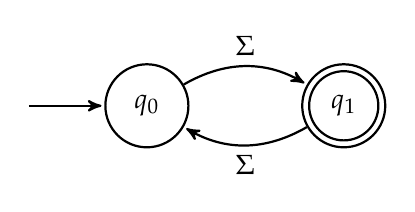
\begin{tikzpicture}[thick, auto]
		\node[main node] (A) {$q_0$};
		\node[main node] at (2.5,0) (B) {$q_1$};
		\node[main node, minimum size=2.5em] at (2.5,0) (Bfin) {};

		\path (A) edge[bend left=30] node {$\Sigma$} (B);
		\path (B) edge[bend left=30] node {$\Sigma$} (A);
		\path (-1.5,0) edge node {} (A);
	\end{tikzpicture}
	\end{center}

	So that for each word in the language $\Sigma$ there exists 
	both a transition from \textit{$q_0$} to \textit{$q_1$} and from 
	\textit{$q_1$} to \textit{$q_0$}.

	\section{Let \textit{A} denote the language that consists of strings 
	with a correct checksum}

	\begin{itemize}
		\item[a)] Proof that $w^R \in A$ for all $w \in A$.

			We see that since $w \in A$ and 
			\[w = a_1a_2...a_nc\]

			so that 

			\[c = a_1 \oplus a_2 \oplus ... \oplus a_n\]

			In the case with $w^R = ca_na_{n-1}...a_2a_1$ we see
			that for $w^R$ to be in $A$, $a_1$ has to be a 
			correct checksum, that is,

			\[a_1 = c \oplus a_n \oplus ... \oplus a_2\]

			And according to our definition of $c$ we get

			\[ c \oplus a_n \oplus a_{n-1} \oplus ... \oplus a_2\]
			\[= a_1 \oplus a_2 \oplus ... \oplus a_n \oplus 
				a_n \oplus a_{n-1} \oplus ... \oplus a_2\]

			We observe here that since $a \oplus a = 0$ we 
			see that each duplicate $a_i$ cancels each other 
			out of the equation and we are left with:

			\[ = a_1 \oplus a_n \oplus a_n = a_1 \oplus 0\]
			\[ = a_1\]

			And therefore, $w^R \in A$.

	$\hfill\blacksquare$

		\item[b)] Show that \textit{A} is regular.

		Here we will show a NFA that represents the language 
		\textit{A}.

		Since we need the checksum, or the last symbol, to be 
		dependent on what we have so far, we will alternate 
		between four states, where each one has the possibility 
		to end on the corresponding \textit{c}, or continue further.

		\begin{adjustwidth}{-5cm}{-3cm}
	\begin{center}
	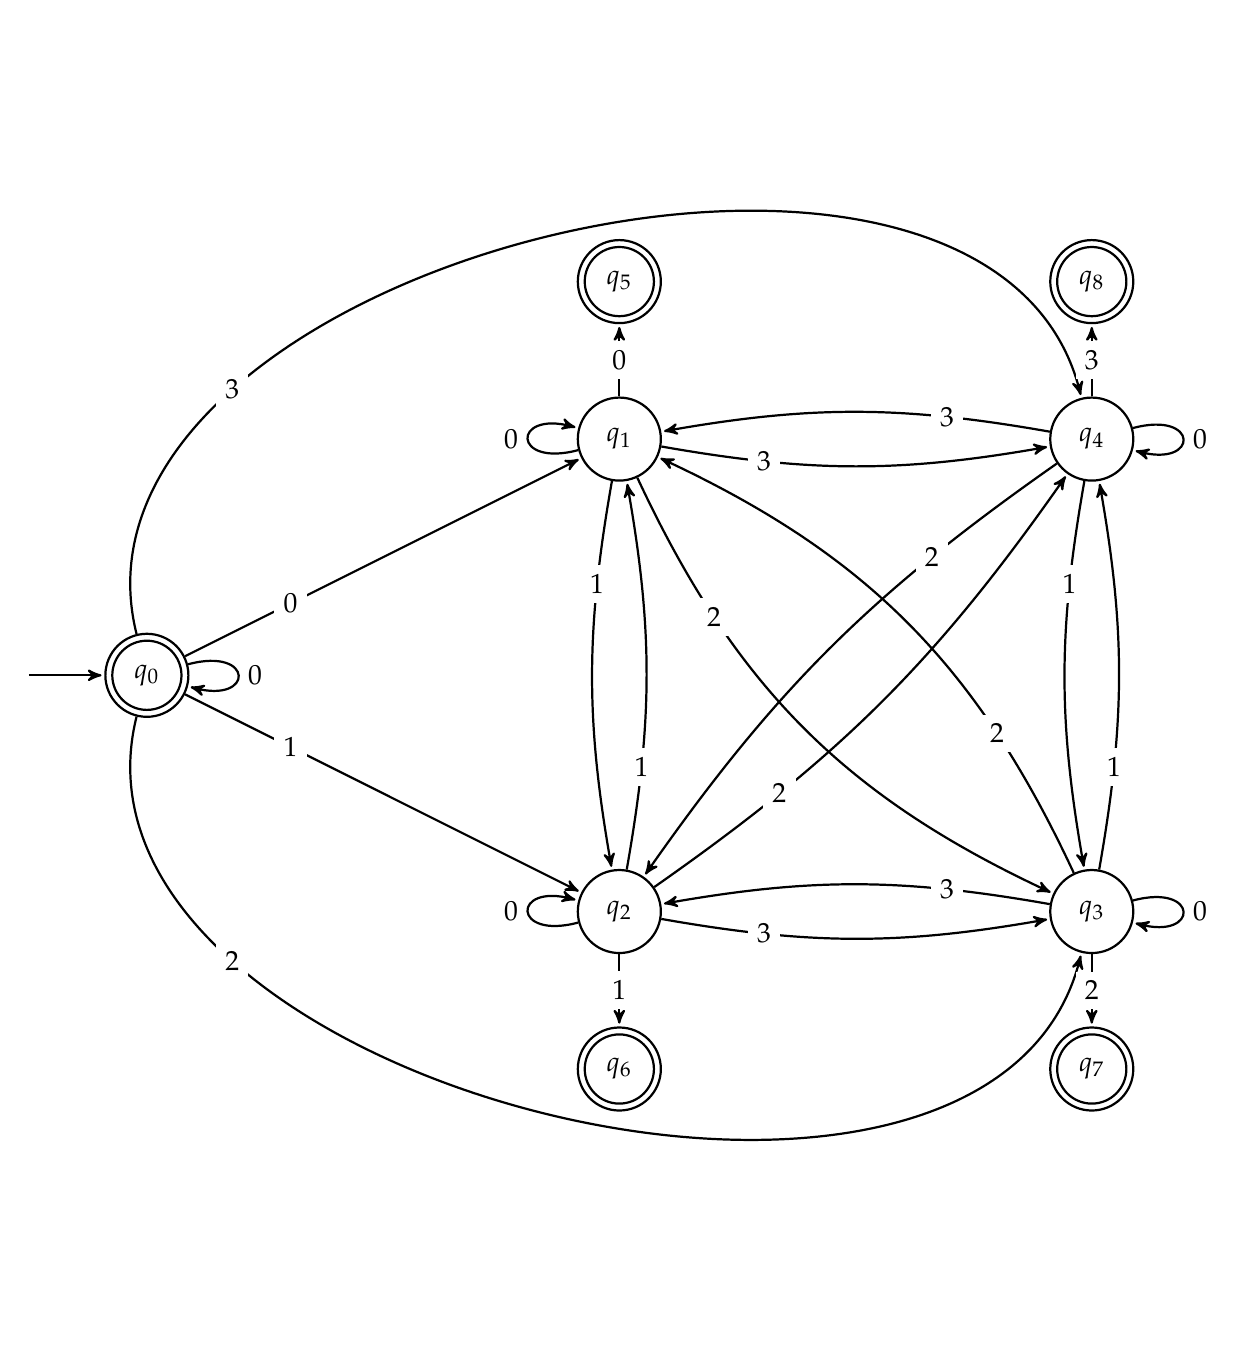
\begin{tikzpicture}[thick]
		\node[main node] at (-5,0) (q0) {$q_0$};
		\node[main node, minimum size=2.5em] at (-5,0) (q0fin) {};
		\node[main node] at (1,3) (q1) {$q_1$};
		\node[main node] at (1,-3) (q2) {$q_2$};
		\node[main node] at (7,-3) (q3) {$q_3$};
		\node[main node] at (7,3) (q4) {$q_4$};

		\node[main node] at (1,5) (q5) {$q_5$};
		\node[main node, minimum size=2.5em] at (1,5) (q5fin) {};
		\node[main node] at (1,-5) (q6) {$q_6$};
		\node[main node, minimum size=2.5em] at (1,-5) (q6fin) {};
		\node[main node] at (7,-5) (q7) {$q_7$};
		\node[main node, minimum size=2.5em] at (7,-5) (q7fin) {};
		\node[main node] at (7,5) (q8) {$q_8$};
		\node[main node, minimum size=2.5em] at (7,5) (q8fin) {};

		\path (q0) edge[bend left=00] node[pos=.25,fill=white] {0} (q1);
		\path (q0) edge[bend right=00] node[pos=.25,fill=white] {1} (q2);
		\path (q0) edge[bend right=90] node[pos=.25,fill=white] {2} (q3);
		\path (q0) edge[bend left=90] node[pos=.25,fill=white] {3} (q4);

		\path (q0) edge[loop right=20] node {0} (q0);
		\path (-6.5,0) edge node {} (q0);

		\path (q1) edge[loop left=10] node {0} (q1);
		\path (q1) edge[bend right=10] node[pos=.25,fill=white] {1} (q2);
		\path (q1) edge[bend right=20] node[pos=.25,fill=white] {2} (q3);
		\path (q1) edge[bend right=10] node[pos=.25,fill=white] {3} (q4);

		\path (q1) edge node[fill=white] {0} (q5);

		\path (q2) edge[loop left=10] node {0} (q2);
		\path (q2) edge[bend right=10] node[pos=.25,fill=white] {1} (q1);
		\path (q2) edge[bend right=10] node[pos=.25,fill=white] {2} (q4);
		\path (q2) edge[bend right=10] node[pos=.25,fill=white] {3} (q3);

		\path (q2) edge node[fill=white] {1} (q6);

		\path (q3) edge[loop right=10] node {0} (q3);
		\path (q3) edge[bend right=10] node[pos=.25,fill=white] {1} (q4);
		\path (q3) edge[bend right=20] node[pos=.25,fill=white] {2} (q1);
		\path (q3) edge[bend right=10] node[pos=.25,fill=white] {3} (q2);

		\path (q3) edge node[fill=white] {2} (q7);

		\path (q4) edge[loop right=10] node {0} (q4);
		\path (q4) edge[bend right=10] node[pos=.25,fill=white] {1} (q3);
		\path (q4) edge[bend right=10] node[pos=.25,fill=white] {2} (q2);
		\path (q4) edge[bend right=10] node[pos=.25,fill=white] {3} (q1);

		\path (q4) edge node[fill=white] {3} (q8);
	\end{tikzpicture}
	\end{center}
	\end{adjustwidth}

	We have then shown that a NFA can be constructed, and therefore
	\textit{A} is regular.

	\end{itemize}

\end{document}
